\documentclass[review]{elsarticle}
\usepackage{graphicx}
\usepackage{url}
\usepackage{amsmath,amssymb,amsfonts}
%\usepackage{algpseudocode}
\usepackage{float}
\usepackage[ruled, linesnumbered]{algorithm2e}
\usepackage{algorithmic}
\usepackage{txfonts}
\usepackage{multirow}
\usepackage{booktabs}
\usepackage{epstopdf}% use pdf format figure
\usepackage{subfigure}
\usepackage{multicol}
\usepackage{txfonts}
\usepackage{bm}
\usepackage{supertabular}
\usepackage{xr}
\usepackage{array}
\usepackage{tabularx}
\usepackage{rotating} %used for "sidewaystable" 
\usepackage{array} %Auto change line in Table
%\usepackage{float}
\usepackage{multirow}
\usepackage{colortbl}

\usepackage{lineno,hyperref}
\usepackage{changepage}
\modulolinenumbers[5]

\journal{Journal of \LaTeX\ Templates}

%%%%%%%%%%%%%%%%%%%%%%%
%% Elsevier bibliography styles
%%%%%%%%%%%%%%%%%%%%%%%
%% To change the style, put a % in front of the second line of the current style and
%% remove the % from the second line of the style you would like to use.
%%%%%%%%%%%%%%%%%%%%%%%

%% Numbered
%\bibliographystyle{model1-num-names}

%% Numbered without titles
%\bibliographystyle{model1a-num-names}

%% Harvard
%\bibliographystyle{model2-names.bst}\biboptions{authoryear}

%% Vancouver numbered
%\usepackage{numcompress}\bibliographystyle{model3-num-names}

%% Vancouver name/year
%\usepackage{numcompress}\bibliographystyle{model4-names}\biboptions{authoryear}

%% APA style
%\bibliographystyle{model5-names}\biboptions{authoryear}

%% AMA style
%\usepackage{numcompress}\bibliographystyle{model6-num-names}

%% `Elsevier LaTeX' style
\bibliographystyle{elsarticle-num}
%%%%%%%%%%%%%%%%%%%%%%%
\begin{document}
	
	\begin{frontmatter}
		
		\title{XXX}
		\author[label1]{Niu Wentao} % nwt001234@gmail.com
		\author[label1]{XXX} % 
		\author[label2]{XXX} %
		\author[label1]{Zhenyu Lei} % leizystu@outlook.com
		\author[label1]{Shangce Gao\corref{cor1}}\ead{gaosc@eng.u-toyama.ac.jp}
		
		\address[label1]{Faculty of Engineering, University of Toyama, Toyama-shi, 930-8555 Japan.}
		\address[label2]{Department of Computer Science and Technology, Beijing University, Beijing 100000, China.}
		%\address[label3]{School of Information and Control Engineering, China University of Mining and Technology, Xuzhou, 221116, China.}
		
		\cortext[cor1]{Corresponding author}
		
		\begin{abstract}
			Medical image segmentation serves as an important tool in the treatment of various medical diseases. However, achieving precise and efficient segmentation remains challenging due to the intricate structures and variations. Although neural network methods based on U-shaped structures have shown impressive results, they often lack effective representation of global-local features, leading to insufficient extraction of multi-scale and contextual information in medical image segmentation tasks. To tackle these challenges, we propose a novel approach: a dilated dendritic model with deep supervision, namely 3DL-Net. It integrates the flexible dilated convolution mechanism into the segmentation architecture, aiming to expand the model’s receptive field and capture richer global features. Additionally, in contrast to other segmentation architectures, we innovatively introduce the processing of  local feature of shallow structures through the dendritic neuron model in medical images into 3DL-Net.  This is the first time dendritic learning has been employed at the channel level and represents a pioneering approach to the local feature process. During the training process, 3DL-Net incorporates a deep supervision mechanism that utilizes our designed loss function. Due to the intermediate supervision signals at various network stages, providing feedback at multiple levels, the model refines its predictions across various scales, contributing to further enhanced segmentation outcomes. To evaluate the effectiveness of our proposed method, we conducted extensive experiments on three medical image datasets to demonstrate significant improvements in segmentation accuracy compared to state-of-the-art models. Our mDice metrics on three datasets achieved 86.61\%, 87.87\%, and 85.06\%, surpassing the second-best models by 3.85\%, 1.54\%, and 0.95\%.

		\end{abstract}
		
		\begin{keyword}
			Medical image segmentation \sep Dendritic learning \sep  Dilated convolution \sep Global-local feature \sep
		\end{keyword}
		
	\end{frontmatter}
	
	%\linenumbers
	\section{Introduction}
	Medical image segmentation plays a crucial role in the accurate extraction and delineation of pathological regions~\cite{iglesias2015multi}. This process enhances the clarity of anatomical or pathological structures within images, aiding in accurate clinical assessments, disease diagnosis, and treatment planning. It plays a significant role in healthcare decision-making and patient care~\cite{duncan2000Medical}. Current medical image segmentation tasks span across various fields and imaging modalities, including computed tomography (CT) and ultrasound. These tasks encompass the segmentation of diverse organs such as the brain, lungs, liver, kidneys, and other vital structures~\cite{shen2017deep,salpea2022medical,antonelli2022medical}.

	In order to help clinicians make accurate diagnoses, segmentation of some key objects in medical images and extraction of features from the segmented region are necessary. Early image segmentation relied on conventional computer vision techniques, such as thresholding~\cite{zhang2006adaptive, senthilkumaran2016image}, edge detection~\cite{chalana1997methodology,mehena2013medical}, region growing~\cite{justice1997medical}, level set~\cite{li2012new}, and graph cut~\cite{boykov2006graph,manoharan2020improved}. These methods utilized specific image features, pixel-level processing, and empirical rules to segment images. Despite the notable contributions of traditional segmentation methods, image segmentation remains one of the most challenging topics in computer vision due to the difficulty of feature representation~\cite{wang2022medical}. In particular, extracting discriminative features from medical images is more difficult than for normal RGB images, since the former are often faced with challenges such as complex background images, noise interference, and variations in target shape~\cite{pham2000current}. Moreover, it further involves managing large volumes of data and addressing issues related to inaccurate location labeling~\cite{hesamian2019deep,scholl2011challenges}. Especially in the clinical process, these challenges become more critical. Clinical specialists seek better methods to address it instead of relying on time-consuming manual procedures for organ segmentation~\cite{mccrindle2021radiology}.

	The emergence of deep learning technologies has effectively addressed challenges such as complex backgrounds, noise interference, and variations in target shape~\cite{xie2021cotr,bao2018multi}, leading to the development of new paradigms. The pivotal paradigm involves eliminating the need for manual crafting of features in medical image segmentation. Convolutional neural networks (CNNs) have emerged as a fundamental tool in medical image segmentation, capable of automatically learning hierarchical features from raw image data. These features encompass a wide range of visual characteristics, including edges, textures, shapes, and other discriminative patterns present in medical images. Due to their insensitivity to variations in image noise, blurring, and contrast, CNNs yield excellent segmentation results for medical images. This relieves healthcare professionals from the laborious task of manually generating features, enabling them to concentrate on directly diagnosing segmented lesion areas. This shift notably enhances the efficiency of clinical diagnosis.

	With the continuous advancement of CNNs, image segmentation technology has achieved significant breakthroughs, particularly in semantic segmentation. Semantic segmentation involves dividing the input image into distinct regions with specific semantic meanings, enabling the identification of semantic categories for each region through pixel-wise annotation~\cite{LATEEF2019321}. Subsequent developments in semantic segmentation methods based on CNNs have introduced notable models such as FCN~\cite{long2015fully}, U-Net~\cite{ronneberger2015u}, and SegNet~\cite{badrinarayanan2017segnet}. However, despite the notable achievements in semantic segmentation using CNN-based approaches, certain challenges persist. One of the primary obstacles involves addressing class imbalance, which refers to the uneven distribution of samples among different classes or regions of interest (ROI)~\cite{japkowicz2002class}. The issue of class imbalance in medical image segmentation often leads to unsatisfactory segmentation results. This challenge becomes evident when minority classes are situated within the ROI, leading to potential neglect or insufficient model learning regarding critical details within these minority categories~\cite{yeung2022unified}. An appropriate loss function constitutes a pivotal approach to mitigating this issue. Conventional loss functions, primarily relying on accuracy, might not effectively address this problem. In response to these challenges, employing specialized loss functions such as Intersection over Union (IoU)~\cite{rezatofighi2019generalized}, focal loss~\cite{lin2017focal}, dice loss~\cite{zhao2020rethinking}, and others for assessing model performance is emphasized.

	Another significant concern is the effective integration of multi-scale and contextual information. It significantly impacts the ability of CNN-based models in various medical image segmentation tasks to comprehend the local image structure and global feature process. Current CNN-based deep learning models often encounter challenges such as the omission of spatial information and insufficient representation of features~\cite{yu2015multi}. The inherent bias of the convolutional layer often restricts the extracted information to the main regions of the segmented area, thus limiting its ability to accurately perceive intricate edge variations and the amalgamation of numerous small segmented regions~\cite{Lv2023Local}. The lack of multi-scale contextual information and the absence of semantic details during pooling operations exacerbate this insufficient feature representation. Notably, medical pathology images demonstrate more significant scale differences in lesion areas compared to typical natural images. Therefore, addressing these challenges necessitates the introduction of more effective multi-scale modules~\cite{srivastava2021msrf}. Specifically, CNN-based methods hierarchically extract features from shallow to deep through convolutional operations. However, these approaches frequently overlook the semantic distinctions between deep and shallow features, making it challenging to capture both global and local features in medical images~\cite{li2022global}. Moreover, traditional CNNs architectures typically prioritize the local receptive field during feature extraction, neglecting the importance of global context information. Therefore, model optimization should involve extracting features across various levels of semantic representations to enhance segmentation tasks. To overcome this limitation, advanced approaches have been introduced, such as incorporating probabilistic graphical models into deep learning architectures~\cite{zheng2015conditional} and utilizing pyramid scene parsing networks (PSPN)~\cite{zhao2017pyramid}. These methods incorporate graph-based and pyramid-based mechanisms to capture multi-scale and contextual information, thereby enhancing the representation of features. Additionally, AAUnet~\cite{chen2022aau}, RRCNet~\cite{chen2023rrcnet}, LEA U-Net~\cite{ouyang2023lea} utilize dilation convolution to expand the receptive field, combining various dilation rates to extract semantic features at different scales. These methods employ dilated convolution to obtain more global features, enabling the model to better capture long-range correlations and global contextual information in the image. Nonetheless, the extraction of coarse-grained features still results in the loss of fine-grained details pertaining to small targets, thereby constraining the performance of their detection. It is essential to propose methods for integrating global coarse-grained and local fine-grained information.

	The introduction of the aforementioned enables the enhancement of segmentation accuracy by simply deepening the network. However, in this process, the significance of shallow features near the output layer is often overlooked. The model may fail to capture some of the finer local structures and characteristics in the image, as they tend to provide relatively surface-level feature representations. Deep features in both natural and medical images exhibit some commonalities, as evidenced by the successful application of models trained on natural images to medical images through transfer learning. Particularly, generic features related to texture and shape are shared~\cite{cheplygina2019cats,karimi2021transfer}. Conversely, shallow features in natural and medical images exhibit substantial content and feature differences. Natural images encompass diverse scenes, emphasizing colors, larger textures, and shapes. In contrast, medical images, where color features are less pronounced, emphasize complex edge contours and focus on depicting the density features hidden within tissues and organ structures. They predominantly highlight characteristics related to grayscale, edges, and shapes. Nevertheless, traditional CNNs networks find it difficult to provide high-precision local feature analysis capabilities~\cite{li2024scribformer}. CNNs usually prioritize the extraction of high-level features while neglecting or inadequately representing low-level features, resulting in the loss of fine-grained details. Moreover, they cannot provide an interpretable basis for segmenting loca features, hindering doctors from giving diagnoses aligned with the underlying pathology. To address these challenges and refine the processing of local features, we propose a novel module for refining local features, introducing the dendritic neuron model (DNM). In contrast to the overly simplistic traditional McCulloch-Pitts model of neurons in CNNs~\cite{mcculloch1943logical}, the DNM represents a biologically plausible model designed to emulate the information processing mechanisms of neurons in the human brain~\cite{gao2018dendritic}. It is introduced to overcome the limitations of traditional artificial neurons, which are often considered too simplistic~\cite{zhou2016financial}. The DNM exhibits robust feature mapping capabilities. Through feature multiplexing and weighting, it can simulate dendritic processes to capture complex, nonlinear relationships, thereby addressing the challenges posed by local features. This approach enables the extraction of subtle local features from shallow representations, thereby enhancing their representation and providing a more interpretable basis for the classification at the final layer.
 
	To meet the challenges in medical image segmentation outlined previously, we propose a novel segmentation method, a dilated dendritic model with deep supervision, 3DL-Net. This method is trained with deep supervision and a loss function tailored for imbalanced class issues. By employing dilated convolutions, 3DL-Net captures broader contextual information, enhancing the representation and understanding of global features. Additionally, the integration of dendritic neurons, a distinct type of neuron from the commonly used McCulloch-Pitts neurons, offers greater biological interpretability and aims to refine the processing and representation of local features with superior precision. The contributions of this work can be summarized as follows:

	\begin{enumerate}[1)]
		\item We leverage dilated convolutions with diverse dilation rates to capture contextual information and multi-scale details from varying receptive fields, thereby obtaining richer representations of global features. This strategy enhances our understanding of the overall structure of surrounding tissues and improves segmentation accuracy for complex boundaries.
		
		\item A novel artificial neuron, DNM, has been introduced and employed at the channel level for the first time to address challenges associated with local feature representation. This approach facilitates the refinement of boundaries and enables superior, precise processing of local features and fine-grained structures.
		
		\item We introduce 3DL-Net, a novel medical image segmentation method designed to address the limitations of representing global-local features. To the best of our knowledge, this is the first attempt to tackle this challenge by leveraging DNM and dilated convolutions. Experimental evaluations demonstrate 3DL-Net remarkable accuracy and robustness, surpassing established state-of-the-art methods in the three public medical image segmentation datasets.
	\end{enumerate}

	The remainder of this paper is structured as follows: Section~\ref{section:rw} provides an overview of relevant literature and previous research in the medical image segmentation field. Section~\ref{section:methodology} details the proposed method in this study. The experimental design and results are discussed in Section~\ref{section:experiment}. Finally, Section~\ref{section:conclusion} presents conclusions and outlines future work.
	
	\section{Related work}
	\label{section:rw}
	\subsection{Medical image segmentation based on deep learning}
 	CNNs have made significant strides in advancing segmentation methods over the years. One of the pioneering models in this field is the FCN~\cite{long2015fully}, which is the first to propose an end-to-end approach for segmentation. It enables pixel-wise classification through fully convolutional layers. This breakthrough brings segmentation tasks into the realm of deep learning and marks the beginning of a new era for image segmentation. Following FCN, the U-Net architecture, proposed by Ronneberger et al.~\cite{ronneberger2015u}, gained popularity for its success in biomedical image segmentation. U-Net is characterized by its U-shaped architecture, which combines contracting and expanding paths to effectively capture both low-level and high-level features. This design has proven particularly valuable in scenarios with limited training data and has been widely adopted in various medical imaging tasks. Another noteworthy model is SegNet~\cite{badrinarayanan2017segnet}, which employs an encoder-decoder architecture with skip connections to reconstruct segmented images while preserving spatial information. This architectural design enables SegNet to better capture the spatial positions of objects and accurately delineate their contours.

	In recent years, inspired by the success of Transformer in computer vision~\cite{vaswani2017attention,chen2021transunet,gu2020net,wang2021transbts}, attention-based visual Transformer methods have been introduced to leverage pixel correlations within medical images, aiming to enhance the effectiveness of medical image segmentation. Initially applied in conjunction with convolutional networks or to replace specific components of such networks, a groundbreaking approach emerged with Dosovitskiy's introduction of the Vision Transformer~\cite{dosovitskiy2020image}. It departs from the reliance on convolutional networks by directly applying the Transformer to sequences of image patches. This departure from traditional convolutional approaches has demonstrated remarkable success in image classification tasks, as evidenced by its excellent performance on various benchmarks. TransUNet~\cite{chen2021transunet} stands out as the pioneer in utilizing a Transformer architecture for medical image segmentation challenges. It ingeniously combines the local feature extraction capability of CNNs with the Transformer's unique ability to capture long-range relationships. Building upon this innovation, SwinUnet~\cite{cao2022swin} further advances the TransUNet framework by introducing a significant modification, substituting the traditional Transformer with a swin Transformer backbone~\cite{liu2021swin}. In this extension, SwinUnet adopts an asymmetric swin Transformer-based decoder with patch expansion layers for efficient upsampling, which aims to restore the spatial resolution of feature maps. In the most recent study, BRAUnet++~\cite{lan2024brau} combines the advantages of CNNs and Transformer to learn global semantic information and minimize local spatial information loss, and amplify the global dimension-interaction of multi-scale features. However, it's important to note that while Transformer models excel at capturing global relationships, there are challenges in handling certain image segmentation tasks, particularly those requiring the detailed analysis of local features. Additionally, in the domain of image processing, pre-training Transformer models may necessitate larger datasets to achieve optimal performance.
	
	\subsection{Segmentation methods through enhancing global feature representation}
	Global features are essential for understanding the contextual information of medical images. While the receptive field of features in the last layer of the network theoretically encompasses a large portion of the input image, in practice, the empirical receptive field is often much smaller. This limitation renders it insufficient to adequately capture global features. Recognizing the limitation of insufficient global feature representation due to limited receptive fields, ParseNet~\cite{liu2016parsenet} introduces global average pooling. This method aggregates the context features from the last layer or any target layer, thereby enhancing the network's ability to capture global context information. By integrating global features into the local feature map, it provides sufficient global context information. However, traditional average pooling only takes into account local information on a fixed scale. As a result, traditional networks are limited to learning a relatively narrow range of feature representations and cannot effectively capture multi-scale features of the image. In addition, pyramid pooling~\cite{zhao2017pyramid} allows the network to comprehensively capture the overall information of an image, including global structure and context at different scales, by extracting feature maps at different scales. 
	
	Pooling is a straightforward and effective method; however, it introduces a potential limitation. The downsampling process may lead to the exclusion of small-sized targets, thereby limiting the network's ability to accurately delineate fine-grained details and small objects within the image. The introduction of dilated convolution solves these problems well while expanding the receptive field. It preserves the image details better and provides a clearer representation of the features. Inspired by this, DeepLab~\cite{chen2017deeplab} utilizes dilated convolutions, also known as hole convolutions, for semantic image segmentation. It achieves an expanded receptive field and captures contextual information at multiple scales by employing dilated convolutions with varying dilation rates, eliminating the need for pooling layers. This allows the model to preserve both spatial resolution and fine-grained details. They subsequently propose a method combining pyramid structure and dilated convolution to further improve the network's ability to perceive multi-scale global information~\cite{chen2018encoder}. Building on this foundation, RRCNet~\cite{chen2023rrcnet} similarly captures more global information by leveraging diverse receptive fields provided by dilated convolution. The difference is that RRCNet incorporates six deep supervised modules to guide the network learning to predict accurate segmentation masks at different scales. It enhances the model's capability to capture both fine-grained details and coarse-grained semantics from features at various scales.
	
	Building upon the aforementioned study, we propose modules designed to enhance the representation of global features. By incorporating dilation convolution with a pyramidal structure and integrating deep supervision into the network, our method improves its representation of global features. However, while dilation convolution expands the receptive field to capture more global information, it may lead to the lost of detailed local features~\cite{hamaguchi2018effective}. Therefore, it is crucial to ensure a more detailed and enriched process for local features while considering the enhancement of global features~\cite{liu2020color}. In this paper, we not only propose modules for enhancing global feature representation but also address the challenges associated with local feature representation through dendritic learning.

	\subsection{Dendritic learning}		
	Traditional artificial neural networks, rooted in McCulloch-Pitts neurons~\cite{mcculloch1943logical}, have been fundamental in shaping the field. Contemporary research is now focusing on architectures that provide increased biological interpretability. One intriguing avenue involves the integration of dendritic neurons, drawing inspiration from the intricate dendritic structures seen in biological neurons~\cite{gao2018dendritic}. Dendrites, the branching extensions of neurons, play a pivotal role in processing incoming neural signals within the brain~\cite{richards2019deep}. The conceptual utility of dendrites in neuroscience underscores the limitations of traditional neuron description, which neglects dendrites' computational properties~\cite{LARKUM20224,tang2022adopting}. The complexity of neuronal behavior surpasses simple point neuron descriptions by including dendrites in their design for a more efficient capture of their true function and the crucial role dendrites play in information processing and overall neural complexity.
	
	Emulating the adaptive behavior of dendrites, dendritic neurons aim to overcome limitations in traditional neural network architectures by effectively capturing local features. The concept of dendritic learning has emerged as a compelling research direction, aiming to incorporate the advantages of biological neurons into artificial intelligence. Consequently, the incorporation of dendritic learning into deep learning models has shown promise in various domains, including image classification, object recognition, and natural language processing~\cite{ji2022survey}. By developing artificial dendrites, Li et al.~\cite{li2020power} present a novel fully integrated neural network with synapses, dendrites, and soma, demonstrating significant improvements in capturing local features and overall performance, particularly in terms of reduced power consumption and improved accuracy in tasks like digit recognition. Egrioglu et al.~\cite{egrioglu2022recurrent} propose a new recurrent dendritic neuron model artificial neural network with a particle swarm optimization-based training algorithm, demonstrating superior forecasting performance in time series prediction. Gao et al.~\cite{gao2021fully} introduce a complex-valued dendritic neuron model by extending DNM from a real-valued domain to a complex-valued domain. Moreover, numerous research endeavors have integrated the notable capability of dendritic networks in effectively addressing nonlinear problems, resulting in improved accuracy and robustness in the field of image classification~\cite{zhang2024dendritic,li2023dendritic,liu2021dendrite}.

	Inspired by the structure and function of retinal ganglion cells, dendritic networks are considered to be a more biologically plausible type of artificial neuron~\cite{zhang2024dendritic,bas2024robust,koch1982retinal}. The design of such neural networks fits with the need for interpretability in medical imaging tasks~\cite{zhang2024lightweight}. However, although dendritic networks have demonstrated excellent performance in a wide range of fields, their application to image segmentation tasks is still relatively limited. We aim to further optimize the structure of dendritic networks to better suit the needs of such tasks. We propose modifying the synapse, dendritic, and soma layers of the dendritic network to incorporate channel-level features, thereby enhancing its applicability to image segmentation tasks. We aim to address specific challenges in medical image analysis, such as accurate delineation of structures and refining the processing of local features, by optimizing the structure of dendritic networks for image segmentation tasks.

	\begin{figure}[t]
		\centering
		\begin{adjustwidth}{-3.5cm}{}
			\includegraphics[scale=0.8]{3DL_architecture.pdf}
		\end{adjustwidth}
		\caption{The basic framework of 3DL-Net, the instance in DSNet and DMNet and the feature maps in the DNM module are the result under random selection.}
		\label{fig:3DL}
	\end{figure}

	\section{Methodology}
	\label{section:methodology}
	\subsection{Architecture of 3DL-Net} 
	This section provides a detailed exposition of our proposed method. It combines three integral modules: the preliminary segmentation module with deep supervision based on variant SegNet (DSNet), the multi-scale contexual module for missed lesions area detection (DMNet), and the shallow feature process utilizing DNM. Each section provides a detailed explanation of these components, with the architecture of 3DL-Net shown in Figure~\ref{fig:3DL}.
	
	The initial step of our segmentation process employs the DSNet module, which conducts the preliminary segmentation of the input medical images. Subsequently, the output of DSNet is fed into DMNet, which specializes in detecting and rectifying missed segmentation regions, further refining the segmentation results. By integrating multi-scale features using dilated neural networks, we can effectively capture fine-grained details and semantic information in images, enhancing adaptability to structures of various sizes and shapes in medical images. This integration also improves the representation and understanding of global features, providing a comprehensive view of the image context and relationships. Throughout the entire segmentation process, DNM plays a pivotal role by cascading at the end of DSNet and DMNet. The shallow features of the two modules are further refined to obtain a richer local feature representation.

	\subsection{Preliminary segmentation module with deep supervision based on variant SegNet} 
	As previously mentioned, the segmentation networks for medical images require the ability to process global-local features. The utilization of multi-scale information at different network levels to enhance global feature representation is an effective method. The shallow layers of the network mainly learn the edge and color information of the image, while the deep layers are responsible for capturing higher-level semantic details. Therefore, it is beneficial to leverage layers of varying scales and integrate highly semantic multiscale feature maps. In addition, extracting location information of anatomical structures or abnormalities from different imaging modalities in medical imaging, including CT, ultrasound, and MRI, can significantly improve the accuracy and reliability of segmentation results~\cite{aljabri2022review}. This information provides contextual information about the entire image, which contributes to the extraction of global features.
	
	In consideration of these issues, we employ SegNet~\cite{badrinarayanan2017segnet} as the backbone. SegNet has a concise yet effective encoder-decoder structure that enables efficient extraction of features from images and captures highly semantic multiscale information. The decoder in the SegNet network recovers spatial information by performing accurate up-sampling using a max-pooling index. Skipping connections enhances context capture by integrating features from different levels of encoders and decoders while preserving spatial information. This is also beneficial for processing local features, as it allows the network to better understand the relationship between the local features and the context information. These superiorities are an explicit response to the challenges faced by backbone networks. 
	
	Building on this, incorporating deep supervision into the method further enhances the feature representation and extraction capabilities of the network. As indicated in Figure~\ref{fig:3DL}, DSNet inserts supervision signals at various levels of the decoder hierarchy; deep supervision guides the learning process of the backbone network. This guidance encourages the generation of multi-scale features, enabling the backbone network to effectively capture both local and global information from medical images~\cite{fu2023deep}. Moreover, DSNet extends the original SegNet architecture by introducing an additional middle layer. It is utilized as the first output for deep supervision, providing an initial coarse result. This improvement allows the network to receive additional supervision signals at an early stage of feature extraction, facilitating the learning process and improving the network's ability to capture both local and global features effectively.
	\begin{figure}[!t]
		\centering
		\begin{adjustwidth}{0cm}{}
			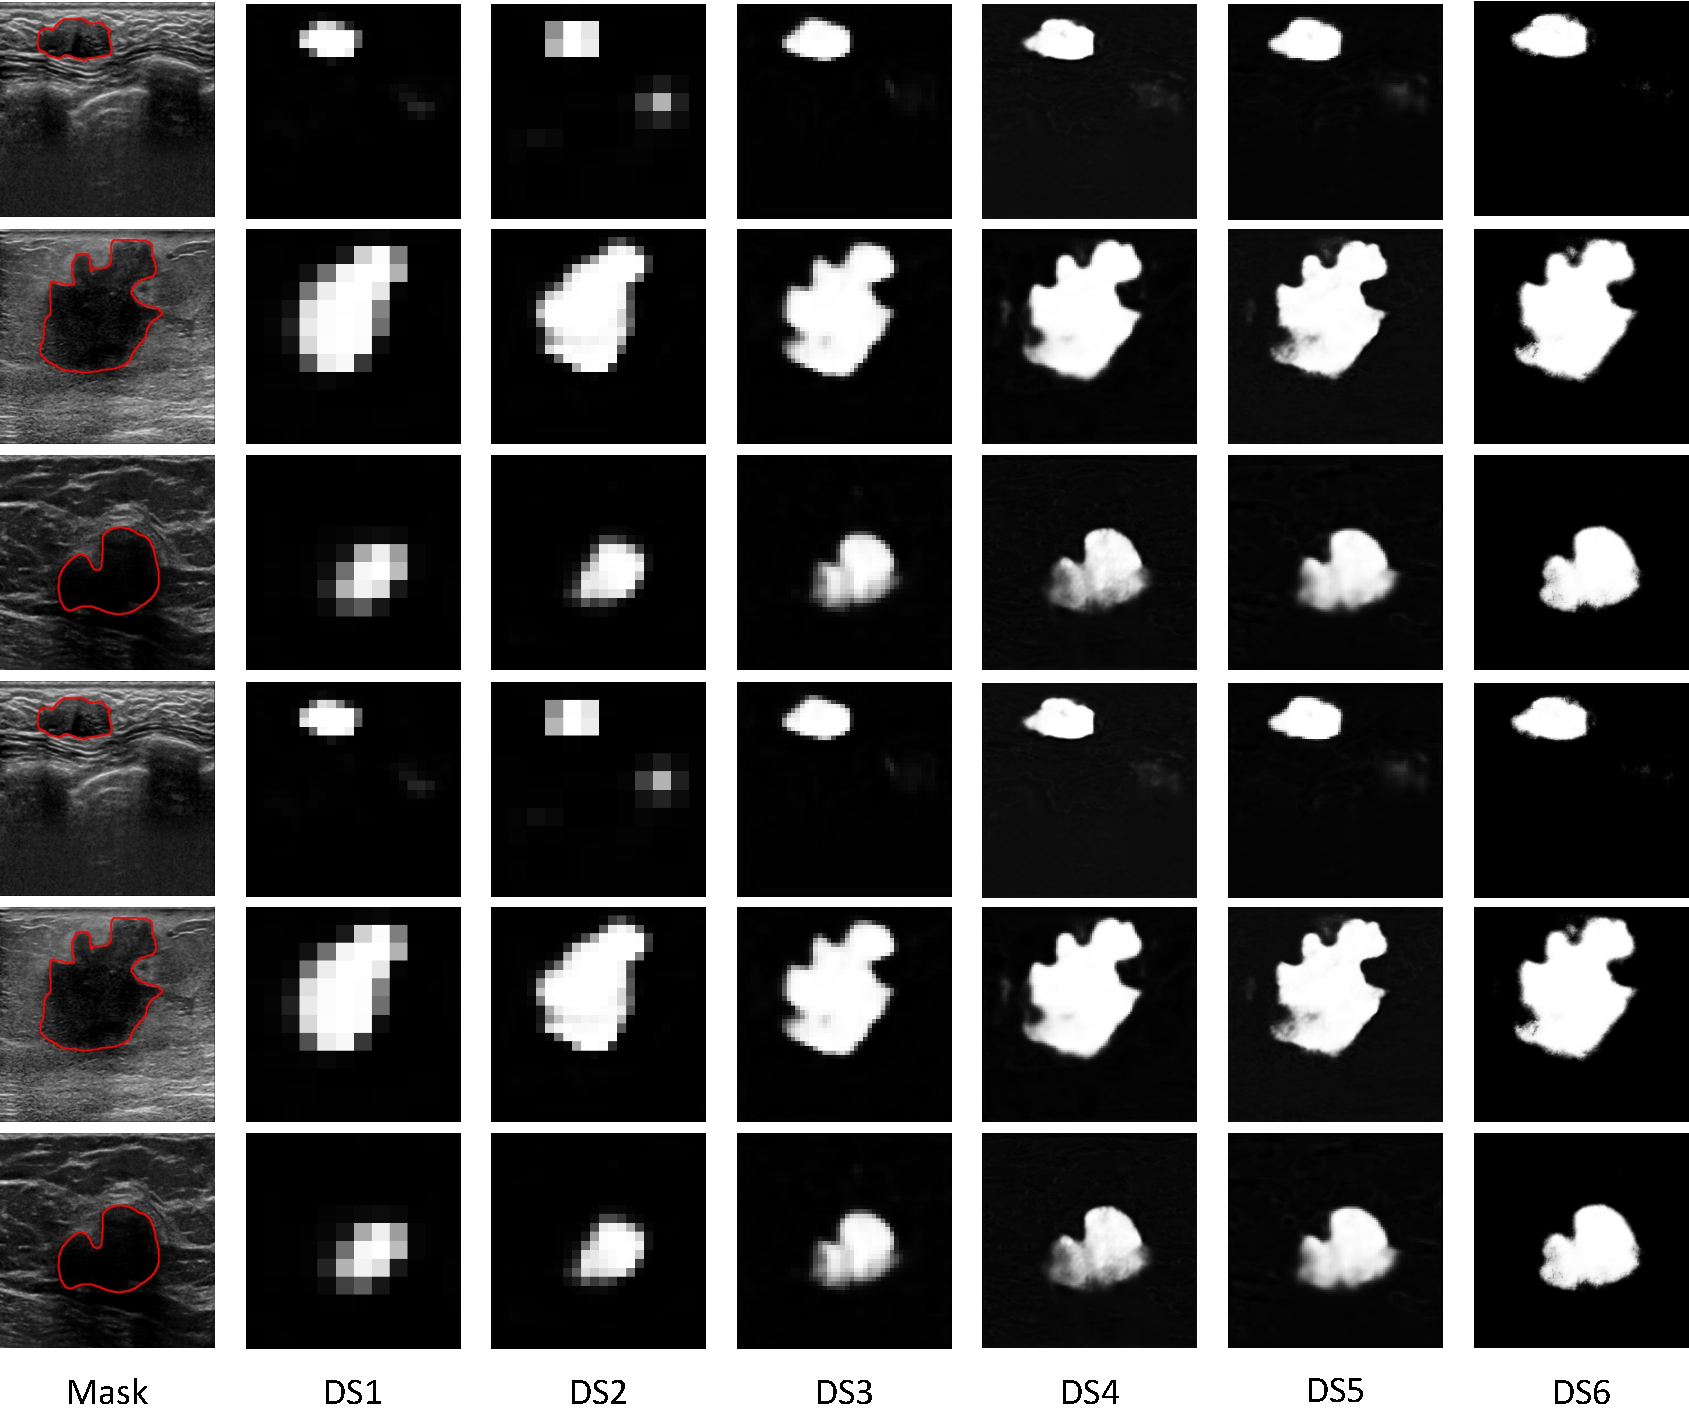
\includegraphics[scale=0.42]{ds.pdf}
		\end{adjustwidth}
		\caption{The visualization of deep supervision.}
		\label{fig:DS}
	\end{figure}
	As illustrated in Figure~\ref{fig:DS}, DSNet produces multiple segmentation masks by introducing the deep supervision module: DS1 for the additional intermediate layer, DS2 for the intermediate layer, and DS3, DS4, and DS5 for each layer of the upsampling process. For each output mask, the feature map's size is initially upsampled through nearest-neighbor interpolation to restore the resolution, facilitating comparison with the original image. Subsequently, these masks undergo dimension reduction and normalization to obtain pixel-level probabilities. The final mask result, DS6, encompasses more comprehensive feature information with higher confidence. Consequently, DS6 is considered the final output of DSNet and acts as the input for the next stage.

	\subsection{Multi-scale contexual module for missed lesions area detection}
	In medical image segmentation, one of the challenges is the lack of contextual information and global features at different scales. This deficiency may lead to the presence of missed detection areas in the medical segmentation task, as factors such as image noise, variability in tissue appearance, or artifacts could disrupt the process. In addition, the CNN-based method may fail to accurately capture these larger lesions due to its limited perception field and may overlook certain areas of interest. For instance, tumors in the middle and later stages tend to be larger in size compared to those in the early stages. Furthermore, when upsampling and downsampling, spatial information may be lost due to the encoder-decoder structure.
	
	In response to these challenges, we propose the DMNet. The size of the perceptual field essentially dictates the extent of contextual information that can be effectively utilized~\cite{wang2022medical}. Larger receptive fields can bring about a richer representation of global features. Inspired by this, DMNet extends the DSNet architecture by incorporating a missed lesions area detection module based on dilated convolution. It enhances sensitivity to missing lesion areas or fine anatomical details through multi-scale capabilities. Besides, it is beneficial to address the limitation of missing spatial information and inadequate representation of global features, which enables more effective detection and aggregation of spatial information at different scales.
	
	\begin{figure}[t]
	\centering
	\begin{adjustwidth}{2.1cm}{}
		\includegraphics[scale=0.18]{ablation.eps}
	\end{adjustwidth}
	\caption{The visualization results of DSNet and DMNet.}
	\label{fig:dilated}
	\end{figure}

	Figure~\ref{fig:dilated} displays distinct components: the labeled region corresponding to the lesion area in the breast cancer image, the prediction outcomes generated by DSNet, the prediction masks by DMNet, and the ultimate composite prediction masks. Owing to the initial predictions from DSNet, there are numerous undetected areas within the lesion region. We develop DMNet to integrate dilation convolution with varying dilated rates, with the goal of capturing the residuals of the lesion region. It results in segmentation with more complete details.
	
	Inspired by the PSPN~\cite{zhao2017pyramid} and dilated convolutions~\cite{chen2017deeplab}, we leverage a pyramid structure and dilated convolutions to effectively capture global features and contextual information at multiple scales, aiming to address the challenges of spatial information loss and inadequate representation of global features in medical image segmentation tasks. Figure~\ref{fig:3DL} The first three blocks of ResNet50 are used in their original structure, while the last block utilizes dilation convolution with a dilation rate set to 2. the architecture of DMNet, specifically, this module first consists of an initial feature extraction branch composed of the residual block. The first three blocks of ResNet50 are used in their original structure, while the last block utilizes dilation convolution with a dilation rate set to 2. Additionally, there are five branches of 3 $ \times $ 3 dilated convolutions with different dilation rates, followed by a final branch of DNM. After receiving the feature outputs from DSNet, DMNet initiates feature extraction through the initial feature extraction branch, resulting in five feature maps. DMNet then combines the extracted features from different scales and levels of abstraction by concatenating these maps. Subsequently, the missed lesion areas identified by DMNet are obtained through the DNM module. Our method fuses these areas with the preliminary rough segmentation results from DSNet to refine the final prediction mask.
	
	The pyramid structure of DMNet facilitates the extraction of both global and local features across multiple scales. This improves the model's ability to recognize lesion areas and structures of different sizes. Additionally, it effectively addresses the challenge of losing global feature information during the continuous downsampling process of the encoder through dilated convolutions. Each layer employs diverse dilation rates to attain varied receptive fields for capturing multi-scale information. This structure enables small convolutional kernels to capture fine features, while large convolutional kernels can extract large-scale features. This aids in effectively detecting the lesion region by comprehensively grasping structures and features in the image. 
	
	Notably, besides the enhancements in network structure, we employ dendritic learning instead of a 1$ \times $1 convolution function at the output of both DSNet and DMNet to achieve the final feature mapping. Further details on the specific implementation of DNM and the visualized feature map will be provided in the next section.

	\subsection{Dendritic neuron module}
	\label{section:updating}
	To enhance the performance of the backbone and effectively map the feature information after rich local feature extraction, we introduce the DNM module. It compensates for the lost of local feature information caused by the larger receptive field introduced by the dilated convolution. As illustrated in Figure~\ref{fig:3DL}, both DSNet and DMNet incorporate our proposed DNM module.
	
	In contrast to prior research~\cite{li2023dendritic,zhang2024dendritic,NING2022108873}, our method concentrates on optimizing the convolution and introduces an additional preprocessing step to enhance the utilization of the dendritic layer. The input image undergoes operations, such as convolutional and pooling layers, within the segmented backbone network. These operations produce a set of maps containing high-level features, which are subsequently utilized for dendritic learning. These features represent an abstract understanding of the complex shape and texture information pertaining to the lesion region in the image. 
	
	To incorporate dendritic learning into the model using a convolution-like approach, we reshape the utilization method of dendritic layers. Initially, we perform multiple dimensionality transformations on input features. Subsequently, we apply layer normalization to these features, ensuring optimal data scaling within the appropriate range. The input data is guided to the synapse layer, where input feature vectors are replicated along channel dimensions to correspond with the number of dendritic branches, promoting desired feature reuse. Following feature reuse, the feature maps undergo initial processing in the synapse layer, involving multiplexing and weighting. This process yields multiple sets of feature maps that more effectively capture the input image features. The processing in the synapse layer can be formulated as follows:
	\begin{equation}
		S_{ij} = \text{ReLU}(k \cdot (w_{ij} \cdot \text{Norm}(x_i) - q_{ij}))
		\label{eq_1}
	\end{equation}
	Here, $S_{ij}$ represents the output of the $j$-th dendritic branch corresponding to the $i$-th element in the input vector $x$. The computational process involves element-wise multiplication between the weights $w_{ij}$ and the input $x$, followed by subtraction of the threshold $q_{ij}$. Subsequent to this operation, the rectified linear unit (ReLU) activation function is applied, introducing non-linearity. The ReLU activation function serves to rectify negative values, thereby preserving salient features, attenuating noise, and disregarding extraneous information. The amplification of the resultant signal is modulated by the parameter $k$. Equation~\ref{eq_1} encapsulates the crux of information integration and processing within the dendritic layer. The learnable parameters, including $k$, $w_{ij}$, and $q_{ij}$, are randomly initialized in the range $(0, 1)$.

	% dendritic layer
	After the individual feature maps $S_{ij}$ traverse the synapse layer, they are subsequently channeled into the dendritic layer. Within this layer, each feature map undergoes a concatenated addition computation, skillfully orchestrated by the dendritic layer. In this intricate process, the $j$-th dendritic branch adeptly consolidates the $N$ input signals $S_{ij}$, culminating in the following computation:
	\begin{equation}
		D_j = \sum_{i=1}^{N} \text{Norm}(S_{ij})
	\end{equation}
	In this expression, $D_j$ serves as the symbolic representation of the amalgamated output emanating from the $j$-th dendritic branch, encapsulating the synergized information gleaned from the $N$ input signals.

	% membrane layer
	Following the intricate computations in the dendritic Layer, the subsequent stage involves the membrane layer which autonomously oversees the segmentation prediction process across multiple layers. In this phase, the membrane layer accumulates the signals from all dendritic branches. Through a summation operation, this layer combines the outputs of the $M$ dendritic branch representation, denoted as:
	\begin{equation}
		O = \sum_{j=1}^{M} D_j
	\end{equation}
	Here, $O$ symbolizes the profound integration of inputs derived from the intricate processes within the dendritic layer, ultimately representing the collective output of this stage.

	The soma Layer concludes the processing pipeline by generating the final prediction. Employing a sigmoid activation function, it processes the output of the membrane layer. Yields the final output prediction $P$ according to the equation:
	\begin{equation}
		P = \frac{1}{1 + e^{-k_s(Y - q_s)}}
	\end{equation}
	Here, $k_s$ and $q_s$ represent additional learnable parameters, initially set randomly within the range of $(0, 1)$. Throughout the training phase, the optimization of these learnable parameters is facilitated by the Adam optimizer.

	The introduced DNM module empowers shallow feature processing, enabling the acquisition of finer local feature representations and more accurate segmentation masks in medical image segmentation tasks. This refinement of local features effectively addresses the issue of loss of fine-grained details in shallow features of medical image segmentation, providing a biologically plausible and interpretable basis. The challenge of losing local feature information due to the large receptive fields introduced by dilated convolution in DMNet is effectively mitigated. In Figure~\ref{fig:feature}, input feature maps are preprocessed and passed through the synapse layer, resulting in $ M $ groups of enriched shallow features. Each group then undergoes processing by the dendritic and membrane layers to produce $ M $ middle feature maps. Finally, the soma layer integrates the middle feature maps to generate the final prediction results. The DNM module executes nonlinear feature mapping, enhancing the model's capacity to capture intricate details and fine-grained structures in medical images, thereby improving segmentation accuracy.

	\begin{figure}[t]
		\centering
		\begin{adjustwidth}{-2.9cm}{}
			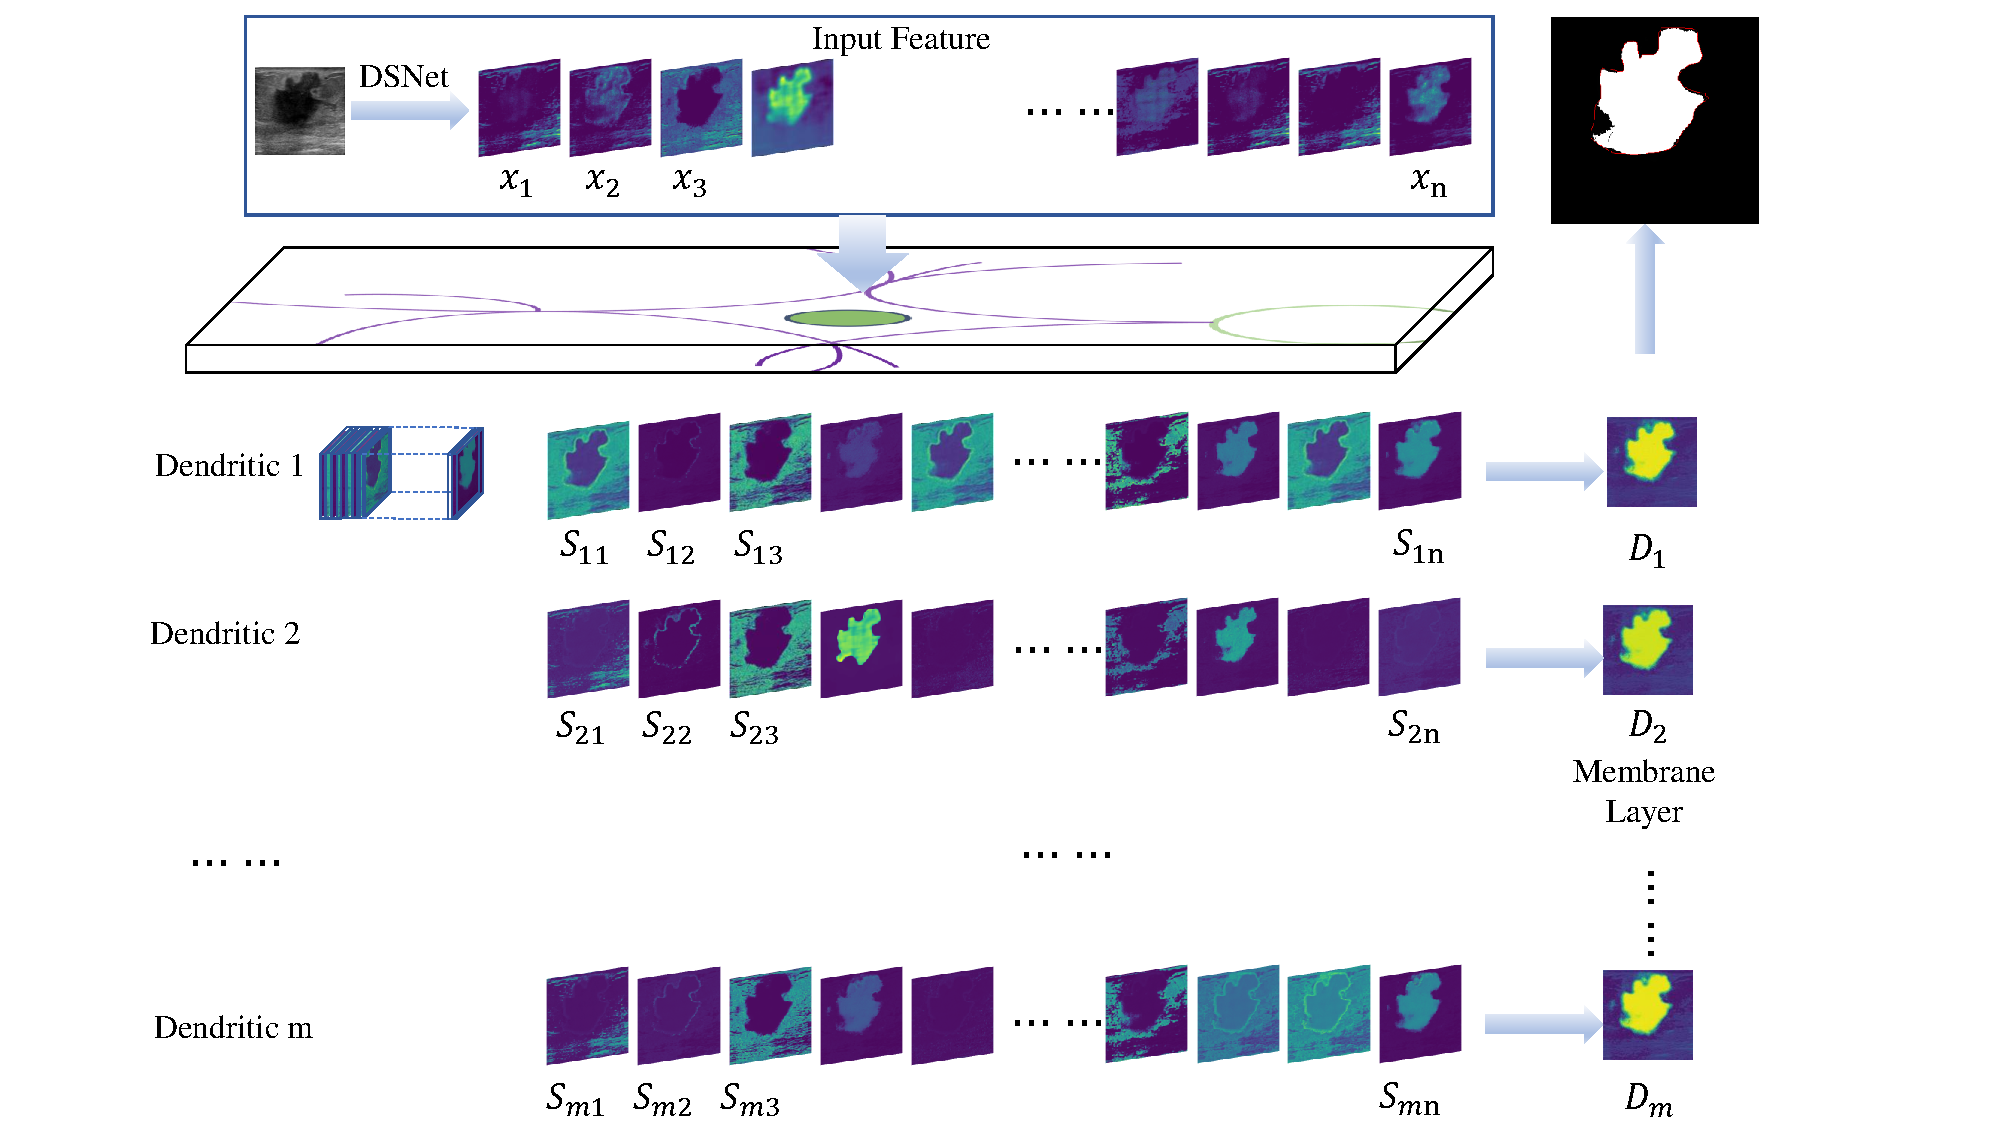
\includegraphics[scale=0.6]{feature.pdf}
		\end{adjustwidth}
		\caption{Visualization of the shallow feature processing of DNM.}
		\label{fig:feature}
	\end{figure}
	
	\subsection{Loss function}
	During the training, a combined loss function incorporating Binary Cross-Entropy Loss (\(\mathcal{L}_\text{BCE}\)) and Self-Adaptive Focal Loss (\(\mathcal{L}_\text{a-Focal}\)) is proposed. This choice arises from the suitability of BCE for pixel binary classification tasks and focal loss for segmentation tasks. It can focus more on hard or misclassified pixels and alleviate class imbalance. The proposed self-adaptive nature of our \(\mathcal{L}_\text{a-Focal}\) is designed to address challenges specific to medical segmentation by dynamically adjusting weights based on the proportion of lesion areas in different data samples.
	\(\mathcal{L}_\text{BCE}\) is given by:
	\begin{equation}
		\mathcal{L}_\text{BCE} = -\frac{1}{N} \sum_{i=1}^{N} \left(t_i \cdot \log(p_i) + (1 - t_i) \cdot \log(1 - p_i)\right)
	\end{equation}
	where \(N\) is the total number of pixels, \(t_i\) represents the ground truth label for pixel \(i\), and \(p_i\) represents the predicted probability.
	
	\(\mathcal{L}_\text{a-Focal}\) is designed to alleviate the challenges caused by uneven distribution of classes and is formulated as follows:
	\begin{equation}
		\mathcal{L}_\text{a-Focal} = -\frac{1}{N} \sum_{i=1}^{N} \alpha_i \cdot (1 - p_i)^{\gamma_i} \cdot \log(p_i)
	\end{equation}
	where \(\alpha_i\) is dynamically adjusted based on the confidence level, and \(\gamma_i\) serves as a focal factor adjusting the loss based on the predicted probability \(p_{g_i}\).
	\begin{equation}
		\gamma_t = (1 - p_g) \cdot \mathbb{I}_{0.15 \leq p_g \leq 0.85} + 0.85 \cdot \mathbb{I}_{p_g = 0.15} + 0.15 \cdot \mathbb{I}_{p_g = 0.85}
	\end{equation}
	This expression defines the focal factor $\gamma_t$ used in the \(\mathcal{L}_\text{a-Focal}\). It adjusts the loss differently based on the predicted probability $p_g$. Specifically: When $p_g$ is within the range [0.15, 0.85], $\gamma_t$ is set to $1 - p_g$, emphasizing learning from examples that are more uncertain (closer to 0.5). When $p_g$ is within the range [0, 0.15], $\gamma_t$ is fixed at 0.85, giving more emphasis to examples predicted with high confidence as positive. When $p_g$ is within the range [0.85, 1], $\gamma_t$ is fixed at 0.15, providing more emphasis to examples predicted with high confidence as negative. This configuration is designed to mitigate overfitting issues associated with unbalanced samples, particularly when the lesion area varies significantly in size.
	
	The final combined loss, denoted as \(\mathcal{L}\), aggregates \(\mathcal{L}_\text{BCE}\) and \(\mathcal{L}_\text{a-Focal}\) for deep supervision, weighted by a factor \(k\):
	\begin{equation}
		\mathcal{L} = \sum_{i=1}^{N} \mathcal{L}_\text{BCE} + k \cdot \sum_{i=1}^{N} \mathcal{L}_\text{a-Focal}
	\end{equation}
	The weighting factor, denoted as $ k $, enables nuanced adjustment in emphasizing the \(\mathcal{L}_\text{a-Focal}\) component. This parameter plays a key role in striking a balance between the two final segmentation loss results and the intermediate auxiliary segmentation loss results embedded in our proposed loss function. This parameter serves as an adaptive adjustment between pixel-wise binary classification and addressing the imbalance in segmentation weights. Through the modulation of $ k $, we exercise control over the relative impact of each loss component during the overall training process. A higher $ k $ accentuates the influence of the \(\mathcal{L}_\text{a-Focal}\), customized to address segmentation challenges by dynamically adapting to variations in lesion area proportions. Conversely, a lower $ k $ prioritizes the (\(\mathcal{L}_\text{BCE}\)), enhanced for pixel-wise binary classification weighting. This nuanced control through the parameter $ k $ provides researchers and practitioners with a flexible mechanism to refine the model's learning objectives, allowing them to formulate the weight tailored to the specific requirements of their medical image segmentation tasks. Experimentation with diverse $ k $ values facilitates the optimization of the network's performance in alignment with the dataset nuances and segmentation goals.
	
	\section{Experiment}
	\label{section:experiment}
	\subsection{Datasets and implementation details}
	To evaluate the effectiveness of 3DL-Net in medical image segmentation, a comprehensive set of experiments is conducted on three widely used public datasets. This section provides details on the experimental datasets, setups, comparative experiments, ablation experiments, parameter discussions, and visualization of the results. 

	The study utilizes three published datasets: the moderately-sized Breast Ultrasound (BUS) dataset~\cite{yap2017automated}, a significantly smaller subset of the BUS dataset (STU)~\cite{zhuang2019rdau}, and a relatively larger COVID-19 dataset~\cite{maftouni2021robust}. The inclusion of diverse medical imaging modalities, including CT and ultrasound, in these datasets highlights the generalizability and robustness of our proposed method. The first dataset is the BUS dataset, collected in 2012 from the UDIAT Diagnostic Centre of the Parc Taulí Corporation, Sabadell (Spain), utilizing a Siemens ACUSON Sequoia C512 system equipped with a 17L5 HD linear array transducer operating at 8.5 MHz. The dataset comprises 163 images from various women, with an average image size of 760 $ \times $ 570 pixels. Each image contains one or more lesions. Among the 163 lesion images, 53 depict cancerous masses, while 110 showcase benign lesions. The STU dataset only comprises 42 BUS images, each with an average size of 128 $ \times $ 128 pixels. These images are acquired by the Imaging Department of the First Affiliated Hospital of Shantou University, utilizing the GE Voluson E10 ultrasonic diagnostic system. The final dataset consists of COVID-19 lesion masks and their corresponding frames compiled from three public datasets. The dataset comprises 2729 pairs of images and corresponding ground truth masks. To maintain consistency across datasets, the masks of all various types of lesions have been uniformly mapped to the color white.

	During the experiments, the following hardware and software configurations are employed: Intel(R) Xeon(R) Silver 4110 CPU @ 2.10 GHz, NVIDIA GeForce RTX A6000, and PyTorch 2.1.0 as the backend. To ensure equitable comparisons in training assessments, the COVID-19 dataset is partitioned using a consistent data partitioning strategy, the BUS dataset and the STU dataset are subjected to quadruple cross-validation studies, which are a frequently utilized method in medical image segmentation. The input images are resized to 384 $ \times $ 384 pixels and normalized to a mean value of [0.485, 0.456, 0.406] with a standard deviation of [0.229, 0.224, 0.225]. Additionally, a ResNet backbone pre-trained on ImageNet~\cite{he2016deep} is utilized as the DMNet encoder. In the training phase, a warm-up strategy is adopted, and the Adam optimization algorithm is employed to optimize the network. The initial learning rate is set to $5e-5$, epoch is set to 100, and the batch size is set to 16. The learning rate underwent a warm-up during the first epoch, gradually increasing from a very small value to the set initial learning rate and then decaying slowly.

	To ensure a fair comparison among experiments, each folded cross-validation experiment randomly selected 25\% of the validation data. The best-performing model on the validation set, determined after loss convergence, is utilized for all methods. During the testing process, images is resized to 384 $ \times $ 384 without employing post-processing optimization strategies. To underscore the reliability and authority of our chosen evaluation metrics, we employed established criteria as recommended by prior research~\cite{hoorali2022irunet, chen2023dseu, iqbal2023bts}. Specifically, evaluation of segmentation performance for BUS and pneumonia involved six established metrics: Precision, Recall, mDice, mIou, Specificity, and F1.

	\subsection{Evaluation metrics}
	Drawing from recent work, we leverage comparable segmentation metrics to conduct a comprehensive evaluation of our model. Six evaluation indicators are utilized to assess the model's performance. In this section, we provide a meticulous exposition of each metric.

	In the context of medical image segmentation, the definitions for true positive (TP), true negative (TN), false positive (FP) and false negative (FN) are as follows:

	TP: Pixels are accurately identified as part of the diseased area when the predicted parameter value is above the defined threshold (indicating the presence of the disease).

	FP: Pixels are mistakenly identified as part of the diseased area when, in reality, the predicted parameter value is below the defined threshold (indicating the absence of the disease).

	TN: Pixels are correctly recognized as not part of the diseased area when the predicted parameter value is below the defined threshold (indicating the absence of the disease).

	FN: Pixels representing the disease but incorrectly identified as not part of the diseased area because the predicted parameter value is above the defined threshold (indicating the presence of the disease).

	Precision represents the ratio of TP redictions to all positive predictions, and Recall represents the proportion of TP predictions to all positive ground truth pixels. Specificity assesses the proportion of TN predictions to all negative ground truth pixels. The Jaccard index quantifies the similarity between predicted and ground truth segmentations. The mDice Coefficient, similar to mIou, quantifies the similarity between predicted and ground truth segmentations, particularly focusing on overlapping areas. In the realm of image segmentation, the F1 score serves as a comprehensive metric, amalgamating model accuracy and recall to deliver a holistic evaluation of the model's performance in the segmentation task. These six indicators serve as our benchmarks for evaluating the model. The specific formulas are as follows:
	\begin{equation}
		\text{Precision} = \frac{\text{TP}}{\text{TP + FP}}
		\label{eq_5}
	\end{equation}

	\begin{equation}
		\text{Recall} = \frac{\text{TP}}{\text{TP + FN}}
	\end{equation}

	\begin{equation}
		\text{mDice} = \frac{2 \times \text{TP}}{2 \times \text{TP + FP + FN}}
	\end{equation}

	\begin{equation}
		\text{mIou} = \frac{\text{TP}}{\text{TP + FP + FN}}
	\end{equation}

	\begin{equation}
		\text{Specificity} = \frac{\text{TN}}{\text{TN + FP}}
	\end{equation}

	\begin{equation}
		\text{F1 Score} = \frac{2 \times \text{Precision} \times \text{Recall}}{\text{Precision + Recall}}
		\label{eq_10}
	\end{equation}

	\subsection{Comparative experiments}
	In this subsection, the 3DL-Net model's segmentation outcomes across three datasets are presented, and we conduct a comparative analysis against various medical image segmentation models. Our assessment comprehensively explores the model's learning capability and generalization, considering both quantitative and visualization analysis. For quantitative evaluation, performance metrics, including those in Eqs.(\ref{eq_5}) to (\ref{eq_10}) are employed, comparing the 3DL-Net model with other models. U-Net~\cite{ronneberger2015u}, U-Net++~\cite{zhou2018unet++}, and SegNet~\cite{badrinarayanan2017segnet} are the traditional methods for image segmentation tasks. AttU-Net~\cite{oktay2018attention} is the classical method that introduces the mechanism of attention. Transunet~\cite{chen2021transunet} and BRAUNet++~\cite{lan2024brau} are the classical and state-of-the-art methods based on transformers. AAUNet~\cite{chen2022aau} and RRCNet~\cite{chen2023rrcnet} are state-of-the-art methods that use dilated convolution, and MBSNet~\cite{jin2023novel} is one of the latest methods for medical image segmentation. Additionally, qualitative results are visually presented for each model, accompanied by an in-depth analysis of selected cases. We have highlighted the best results for each metric in bold and the second best in italics. Additionally, we have emphasized the most frequently bolded result, representing the best method, and indicated the second best method with underlining.
	
	\begin{table}[!h]
		\centering
		\caption{The comparison experiment results (mean ± std) in the BUS dataset.}
		\label{table:Contrasting_BUS}
		\begin{adjustwidth}{-4.86cm}{}
			\scalebox{0.87}{                    
				\begin{tabular}{lllllllllll}
					\hline
					Methods            & U-Net             & U-Net++           & AttU-Net                  & SegNet           & TransUNet        & AAUNet           & MBSNet           & BRAUNet++       & \textit{RRCNet}           & \textbf{3DL-Net}                      \\ \hline
					Precision($\%$)    & \underline{88.31 $\pm$ 2.58} & 86.59 $\pm$ 3.12 & 85.27 $\pm$ 4.81 &                                                                                                                                                                                                                  79.70 $\pm$ 3.63 & 80.36 $\pm$ 6.84 & 78.83 $\pm$ 2.40 & 86.93 $\pm$ 0.86 & 84.81 $\pm$ 3.32 & 81.77 $\pm$ 4.12 & \textbf{88.36 $\pm$ 2.03} \\
					Recall($\%$)       & 77.06 $\pm$ 5.74 & 80.44 $\pm$ 2.45 & 75.52 $\pm$ 7.31 & 66.81 $\pm$ 6.24 & 73.53 $\pm$ 7.92 & 82.22 $\pm$ 3.84 & 73.05 $\pm$ 2.36 & 72.31 $\pm$ 1.41 & \underline{82.82 $\pm$ 1.70} & \textbf{85.67 $\pm$ 2.00} \\
					mDice($\%$)        & 81.46 $\pm$ 5.44 & \underline{82.76 $\pm$ 2.79} & 78.27 $\pm$ 4.20 & 72.25 $\pm$ 3.33 & 75.84 $\pm$ 5.66 & 78.14 $\pm$ 2.41 & 78.17 $\pm$ 1.92 & 76.99 $\pm$ 2.17 & 80.40 $\pm$ 2.31 & \textbf{86.61 $\pm$ 0.70} \\
					mIou($\%$)         & 69.55 $\pm$ 7.15 & 71.38 $\pm$ 3.68 & 66.04 $\pm$ 5.03 & 56.85 $\pm$ 4.19 & 61.86 $\pm$ 7.35 & 69.10 $\pm$ 2.98 & 65.53 $\pm$ 1.92 & 63.18 $\pm$ 3.01 & \underline{71.81 $\pm$ 2.74} & \textbf{76.85 $\pm$ 1.04} \\
					Specificity($\%$)  & 99.45 $\pm$ 0.20 & 99.30 $\pm$ 0.24 & 99.36 $\pm$ 0.26 & 99.18 $\pm$ 0.15 & 98.98 $\pm$ 0.50 & 98.82 $\pm$ 0.35 & \underline{99.46 $\pm$ 0.20} & 99.39 $\pm$ 0.13 & 99.01 $\pm$ 0.39 & \textbf{99.52 $\pm$ 0.10} \\
					F1($\%$)           & \underline{84.99 $\pm$ 4.06} & 84.63 $\pm$ 2.84 & 81.48 $\pm$ 2.49 & 75.72 $\pm$ 2.11 & 77.95 $\pm$ 5.40 & 80.49 $\pm$ 2.95 & 82.30 $\pm$ 1.05 & 80.70 $\pm$ 2.60 & 82.29 $\pm$ 2.41 & \textbf{87.47 $\pm$ 1.18} \\ \hline
			\end{tabular}}
		\end{adjustwidth}
	\end{table}
	
	\begin{table}[!h]
		\centering
		\caption{The comparison experiment results (mean ± std) in the STU dataset.}
		\label{table:Contrasting_STU}
		\begin{adjustwidth}{-4.86cm}{}
			\scalebox{0.87}{
				\begin{tabular}{lllllllllll}
					\hline
					Methods            & U-Net             & U-Net++           & AttU-Net                  & SegNet           & TransUNet        & AAUNet           & MBSNet           & BRAUNet++       & \textit{RRCNet}           & \textbf{3DL-Net}                       \\ \hline
					Precision   ($\%$) & 88.28 $\pm$ 4.32 & 87.37 $\pm$ 7.53 & \textbf{90.74 $\pm$ 2.65} & 81.54 $\pm$ 4.08 & \underline{90.35 $\pm$ 1.62} & 89.30 $\pm$ 2.82 & 87.41 $\pm$ 4.81 & 90.03 $\pm$ 2.97 & 88.35 $\pm$ 5.40 & 90.22 $\pm$ 0.36          \\
					Recall      ($\%$) & 84.84 $\pm$ 3.44 & 83.53 $\pm$ 1.27 & 79.33 $\pm$ 6.85          & 85.01 $\pm$ 4.81 & 82.01 $\pm$ 2.01 & 81.66 $\pm$ 5.44 & 85.00 $\pm$ 5.69 & 80.51 $\pm$ 5.65 & \underline{85.32 $\pm$ 3.30} & \textbf{85.71 $\pm$ 3.84} \\
					mDice       ($\%$) & 86.14 $\pm$ 2.35 & 85.08 $\pm$ 3.66 & 84.30 $\pm$ 3.95          & 83.59 $\pm$ 3.39 & 85.97 $\pm$ 1.30 & 85.18 $\pm$ 2.71 & 86.03 $\pm$ 3.46 & 84.84 $\pm$ 2.01 & \underline{86.54 $\pm$ 2.99} & \textbf{87.87 $\pm$ 2.05} \\
					mIou        ($\%$) & 75.89 $\pm$ 3.68 & 74.49 $\pm$ 5.57 & 73.18 $\pm$ 5.99          & 71.97 $\pm$ 5.02 & 75.40 $\pm$ 1.98 & 74.26 $\pm$ 4.05 & 75.74 $\pm$ 5.21 & 73.71 $\pm$ 3.06 & \underline{76.46 $\pm$ 4.68} & \textbf{78.41 $\pm$ 3.23} \\
					Specificity $\%$) & 98.42 $\pm$ 0.66 & 97.93 $\pm$ 1.90 & \underline{98.82 $\pm$ 0.12}          & 97.35 $\pm$ 0.32 & 98.70 $\pm$ 0.25 & 98.57 $\pm$ 0.88 & 98.09 $\pm$ 0.90 & 98.76 $\pm$ 0.70 & 98.40 $\pm$ 0.93 & \textbf{98.83 $\pm$ 0.12} \\
					F1          ($\%$) & 87.17 $\pm$ 3.10 & 86.17 $\pm$ 5.54 & 87.36 $\pm$ 2.58          & 82.53 $\pm$ 3.52 & 88.10 $\pm$ 1.27 & 87.16 $\pm$ 1.94 & 86.68 $\pm$ 3.63 & 87.31 $\pm$ 1.02 & \underline{87.41 $\pm$ 4.00} & \textbf{89.02 $\pm$ 1.08} \\ \hline
			\end{tabular}}
		\end{adjustwidth}
	\end{table}
	
	\begin{table}[!h]
		\centering
		\caption{The comparison experiment results (mean ± std) in the COVID-19 dataset.}
		\label{table:Contrasting_COVID}
		\begin{adjustwidth}{-4.86cm}{}
			\scalebox{0.87}{
				\begin{tabular}{lllllllllll}
					\hline
					Methods            & U-Net             & U-Net++          & AttU-Net          & SegNet           & TransUNet        & AAUNet                    & MBSNet           & BRAUNet++        & \textit{RRCNet}           & \textbf{3DL-Net}                       \\ \hline
					Precision   ($\%$)  & 91.92 $\pm$ 1.81 & \textbf{92.85 $\pm$ 0.81}& 90.84 $\pm$ 1.95 & 89.27 $\pm$ 0.73 & 91.57 $\pm$ 4.17 & \underline{92.74 $\pm$ 0.95} & 91.04 $\pm$ 0.65 & 91.38 $\pm$ 0.57 & 80.43 $\pm$ 1.04 & 82.09 $\pm$ 0.17          \\
					Recall 	    ($\%$)  & 74.77 $\pm$ 1.52 & 74.16 $\pm$ 0.85 & 75.28 $\pm$ 1.63 & 75.40 $\pm$ 0.59 & 62.37 $\pm$ 2.61 & 72.87 $\pm$ 1.12          & 75.83 $\pm$ 0.46 & 70.37 $\pm$ 0.28 & \underline{88.38 $\pm$ 1.14} & \textbf{88.39 $\pm$ 0.18} \\
					mDice       ($\%$)  & 82.27 $\pm$ 0.15 & 82.27 $\pm$ 0.19 & 82.15 $\pm$ 0.24 & 81.48 $\pm$ 0.22 & 73.71 $\pm$ 0.37 & 81.43 $\pm$ 0.34          & 82.53 $\pm$ 0.20 & 79.27 $\pm$ 0.07 & \underline{84.11 $\pm$ 0.07} & \textbf{85.06 $\pm$ 0.03} \\
					mIou        ($\%$)  & 70.09 $\pm$ 0.22 & 70.13 $\pm$ 0.29 & 69.94 $\pm$ 0.35 & 69.14 $\pm$ 0.31 & 58.85 $\pm$ 0.47 & 68.93 $\pm$ 0.47          & 70.51 $\pm$ 0.25 & 66.01 $\pm$ 0.10 & \underline{72.82 $\pm$ 0.12} & \textbf{74.16 $\pm$ 0.04} \\
					Specificity ($\%$)  & 99.86 $\pm$ 0.04 & \underline{99.88 $\pm$ 0.02} & 99.85 $\pm$ 0.03 & 99.84 $\pm$ 0.01 & 99.85 $\pm$ 0.09 & \textbf{99.89 $\pm$ 0.02} & 99.85 $\pm$ 0.02 & 99.86 $\pm$ 0.01 & 99.74 $\pm$ 0.02 & 99.76 $\pm$ 0.00          \\
					F1          ($\%$)  & 82.44 $\pm$ 0.18 & 82.45 $\pm$ 0.21 & 82.30 $\pm$ 0.23 & 81.75 $\pm$ 0.20 & 74.09 $\pm$ 0.42 & 81.60 $\pm$ 0.33          & 82.74 $\pm$ 0.16 & 79.51 $\pm$ 0.07 & \underline{84.25 $\pm$ 0.08} & \textbf{85.12 $\pm$ 0.03} \\ \hline
			\end{tabular}}
		\end{adjustwidth}
	\end{table}	
		
	\subsubsection{Quantitative analysis}

		Table~\ref{table:Contrasting_BUS} illustrates that 3DL-Net achieves a dominant advantage over second place on the BUS dataset. In particular, we improve 5.04\% on mIoU and outperform U-Net++ by about 3.85\% on mDice. Compared to RRCNet, our method achieves a Recall improvement of about 2.85\%, emphasizing lesion detection capability and reducing the risk of missed detection. Our Precision outperformed the closest competitor by approximately 0.05\%. The Specificity of our method outperforms U-Net by approximately 0.07\%. Finally, F1 Score shows a significant improvement, outperforming RRCNet by about 5.18\%. These results demonstrate that our method indeed significantly improves segmentation accuracy on the BUS dataset.
		
		Table~\ref{table:Contrasting_STU} demonstrates the performance on the STU dataset. 3DL-Net performs slightly worse than AttU-Net in Precision, but this metric alone may not provide a comprehensive assessment of segmentation performance. Thus it primarily evaluates the classifier's accuracy in identifying lesion regions. Notably, AttU-Net exhibits significantly lower scores in Recall, mDice, and mIoU. This discrepancy suggests that it may not meet the essential requirements for medical image segmentation. Conversely, our model excels in other metrics, with improvements of 3.32\%, 1.54\%, 4.46\%, 0.01\%, and 2.12\% compared to the second-best results in Recall, mDice, mIoU, Specificity, and F1 Score.
			
		Table~\ref{table:Contrasting_COVID} demonstrates the results of 3DL-Net and contrasting methods on the COVID-19 dataset. Although we have not achieved optimal results on Precision, it's worth noting that mDice may hold more significance in medical image segmentation tasks. This metric emphasizes the discovery and accurate segmentation of positive samples, such as lesions, which is crucial in medical diagnosis~\cite{milletari2016v}. Moreover, mDice inherently combines aspects of both precision and recall metrics. For example, a higher mDice score indicates better overlap between predicted and ground truth segmentation masks, implying both high precision and recall. This is exemplified by the performance of U-Net++, which, despite achieving the best precision, exhibits mediocre performance on several other metrics, suggesting the importance of considering overall segmentation quality rather than focusing solely on precision. In addition, while our Specificity may not rank highest among the metrics, it solely evaluates the model's ability to correctly identify healthy regions (true negatives). Given that healthy regions constitute a significant portion of medical image segmentation tasks, many methods tend to achieve high scores in Specificity. However, relying solely on this metric may not provide a comprehensive assessment of segmentation effectiveness. Therefore, it's essential to consider a diverse range of metrics to accurately evaluate the model's performance in delineating both pathological and healthy regions.
		3DL-Net achieved the best results in other indicators, highlighting our superior capability in lesion detection. It achieves 88.39\% ± 0.18, 85.06\% ± 0.03, 74.16\% ± 0.04, and 85.12\% ± 0.03 in Recall, mDice, mIoU, and F1 Score, with improvements of 0.01\%, 0.95\%, 1.34\%, and 0.87\% compared to the second-best results.
		
		The significant gap between 3DL-Net and existing methods can be explained by the fact that the representation of global-local features has significantly improved. The proposed DMNet is able to obtain multi-scale semantic features at each level. In contrast to the U-Net, SegNet, and U-Net++ that use the same scale feature map in cascade, DMNet helps to preserve finer-grained details. In addition, the proposed DNM module provides more refined processing of local features. The limitation of insufficient local feature representation brought about by the introduction of dilated convolution is also addressed compared to RRCNet and AAUNet. In addition, the standard deviation values in the table indicate that our method exhibits significantly better robustness compared to other methods. This stability is particularly crucial in medical imaging segmentation tasks. It is essential for accurate lesion area detection.
	
	\begin{figure}[!t]
		\centering
		\begin{adjustwidth}{-4.4cm}{}
			\includegraphics[scale=0.18]{DatasetsB.eps}
		\end{adjustwidth}
		\caption{Visual Comparison with State-of-the-Art Methods on BUS dataset. White pixels represent the predicted values, and red curves represent the ground truth values.}
		\label{fig:Visual_BUS}
	\end{figure}
	\begin{figure}[!t]
		\centering
		\begin{adjustwidth}{-4.4cm}{}
			\includegraphics[scale=0.18]{STU.eps}
		\end{adjustwidth}
		\caption{Visual Comparison with State-of-the-Art Methods on STU dataset. White pixels represent the predicted values, and red curves represent the ground truth values.}
		\label{fig:Visual_STU}
	\end{figure}
	\begin{figure}[!t]
		\centering
		\begin{adjustwidth}{-4.4cm}{}
			\includegraphics[scale=0.18]{Covid.eps}
		\end{adjustwidth}
		\caption{Visual Comparison with State-of-the-Art Methods on COVID-19 dataset. White pixels represent the predicted values, and red curves represent the ground truth values.}
		\label{fig:Visual_COVID}
	\end{figure}
	
	\subsubsection{Visualization analysis}
	The visualization results on the BUS dataset are depicted in Figure~\ref{fig:Visual_BUS}. From the visualization images, it is evident that the segmented results exhibit a high degree of similarity to the original ground truth, confirming the accuracy of 3DL-Net. These visualization results highlight the superior segmentation performance of 3DL-Net compared to other methods. Similarly to the quantitative results, the visualization outcomes of each method demonstrate similarities. However, our proposed method demonstrates clear advantages, particularly when built upon the baseline of SegNet. We observe substantial improvements in accurately identifying numerous lesion sites, addressing the limitations of the original SegNet in refining boundaries, and facilitating enhanced delineation of local structures. Compared to U-Net and its variants, 3DL-Net, with its DMNet-enhancing global features, successfully detects many regions that would have been missed by segmentation. Additionally, compared to several state-of-the-art networks, 3DL-Net demonstrates significant improvements in refining boundaries. This improvement can be attributed to the fact that while these networks primarily focus on global feature extraction, they often overlook the issue of a lack of adequate representation of local features due to the inherent characteristics of dilated convolution. Our proposed DNM aims to optimize local feature processing, resulting in enhanced delineation of segmentation boundaries.
	
	The visualization results on the STU dataset are depicted in Figure~\ref{fig:Visual_BUS}. Notably, STU is a small dataset, which poses a challenge due to its limited amount of tumor data, making it difficult for many networks to capture a comprehensive representation of lesion features. The proposed DMNet plays a crucial role in addressing this issue by capturing more global features through an expanded receptive field. This becomes particularly apparent when compared with traditional networks that do not effectively incorporate global features. As a result, BRAUNet++ and RRCNet achieve excellent segmentation results. BRAUNet++ utilizes a hierarchically constructed encoder-decoder architecture along with attention mechanisms to learn global semantic features. RRCNet, on the other hand, utilizes inflated convolution, which expands the receptive field of the network, and deep supervision to guide the learning process at multiple network depths. However, despite their strengths, they lack the capability to refine local features effectively. Thus, 3DL-Net achieves more accurate results in delineating the boundaries of the lesion areas, as it addresses the challenge of refining local features while capturing more global features, leading to superior segmentation boundary details.
	
	The comprehensive and precise segmentation visualization results of lung images provide additional evidence supporting these observations. The visualization results on the COVID-19 dataset are illustrated in Figure~\ref{fig:Visual_COVID}. Compared to other methods, the various approaches demonstrate similar overall structures and layouts. They exhibit comparable efficacy in capturing global features. Due to the intricate nature of the focal area in COVID-19 and the presence of numerous minor lesions, the network faces challenges in accurately identifying numerous small-sized targets. However, 3DL-Net excels in delineating local anatomical structures and capturing fine details. This underscores the effectiveness of 3DL-Net in capturing and leveraging local features, which can be attributed to the meticulous refinement facilitated by our proposed DNM module.

	\subsection{Parameter analysis}
	\label{section:lspa}
	$ k $ is an important parameter in the loss function. Table~\ref{table:Para_k} presents the outcomes of our parameter $ k $ modulation using the BUS dataset, highlighting the optimal segmentation performance achieved with $ k $ set to 0.1. While a value of 0.05 for $ k $ yields excellent results in Precision, Recall is not satisfactory. Notably, the F1 score, which comprehensively balances between Recall and Precision, underscores the superiority of setting $ k $ to 0.1. This specific value of $ k $ strikes the best balance between the (\(\mathcal{L}_\text{BCE}\)) and \(\mathcal{L}_\text{a-Focal}\), yielding the most favorable segmentation outcomes on BUS.

	\begin{table}[!h]
		\centering
		\caption{Parameter analysis results (mean ± std) for parameter $k$ in the BUS Dataset.}
		\label{table:Para_k}
		\resizebox{\columnwidth}{!}{
			\begin{tabular}{lllllll}
				\hline
				$ k $                 & 0.01              & 0.05             & 0.1                       & 0.3              & 0.5              & 0.7            \\  \hline
				Precision   ($\%$)  & 87.28 $\pm$ 4.60  & \textbf{90.06 $\pm$ 2.44} & 88.36 $\pm$ 2.03 & 87.77 $\pm$ 3.08 & 85.29 $\pm$ 3.33 & 85.29 $\pm$ 3.33 \\
				Recall      ($\%$)  & 80.42 $\pm$ 3.87  & 78.70 $\pm$ 4.06 & \textbf{85.67 $\pm$ 2.00} & 78.81 $\pm$ 2.95 & 80.74 $\pm$ 7.37 & 80.74 $\pm$ 7.37 \\
				mDice       ($\%$)  & 82.53 $\pm$ 2.77  & 83.18 $\pm$ 2.65 & \textbf{87.87 $\pm$ 2.05} & 81.83 $\pm$ 1.19 & 81.62 $\pm$ 5.93 & 81.62 $\pm$ 5.93 \\
				mIou        ($\%$)  & 71.56 $\pm$ 3.34  & 71.82 $\pm$ 3.54 & \textbf{76.85 $\pm$ 1.04} & 70.40 $\pm$ 1.67 & 69.80 $\pm$ 8.11 & 69.80 $\pm$ 8.11 \\
				Specificity ($\%$)  & 99.54 $\pm$ 0.05  & \textbf{99.60 $\pm$ 0.14} & 98.83 $\pm$ 0.12 & 99.50 $\pm$ 0.10 & 99.39 $\pm$ 0.21 & 99.39 $\pm$ 0.21 \\
				Accuracy    ($\%$)  & 98.50 $\pm$ 0.52  & 98.47 $\pm$ 0.24 & \textbf{98.75 $\pm$ 0.43} & 98.45 $\pm$ 0.44 & 98.47 $\pm$ 0.50 & 98.47 $\pm$ 0.50 \\
				F1 	        ($\%$)  & 84.80 $\pm$ 3.08  & 86.47 $\pm$ 2.13 & \textbf{87.47 $\pm$ 1.18} & 84.67 $\pm$ 1.46 & 83.37 $\pm$ 4.47 & 83.37 $\pm$ 4.47 \\  \hline
		\end{tabular}}
	\end{table}

	In addition, we conducted a detailed analysis of the parameter $ M $, representing the number of dendrites in dendritic learning. As shown in Table~\ref{table:Para_M} our findings suggest that the choice of $ M $ influences the model's performance in medical image segmentation tasks. Specifically, the model exhibits optimal segmentation performance whlie $ M $ is set to 10, indicating that configuring the network with 10 dendrites is most suitable for effectively capturing microstructures in the feature maps received by the synapses layer in the DNM. However, we also observed that excessively large or small values of $ M $ lead to a decline in performance, highlighting the need to adjust the number of dendrites within a certain range to balance the model's complexity and performance.

	\begin{table}[!h]
		\centering
		\caption{Parameter analysis results (mean ± std) for parameter $M$ in the BUS Dataset.}
		\label{table:Para_M}
		\resizebox{\columnwidth}{!}{
			\begin{tabular}{llllll}
				\hline
				$ M $   		& 1                 & 5                & 10               & 15               & 20               \\ \hline
				Precision($\%$)   & 86.17 $\pm$ 3.10  & 88.19 $\pm$ 5.40 & \textbf{88.36 $\pm$ 2.03} & 87.05 $\pm$ 4.76 & 85.99 $\pm$ 4.70 \\
				Recall($\%$)      & 70.94 $\pm$ 7.02  & 83.44 $\pm$ 3.41 & \textbf{85.67 $\pm$ 2.00} & 79.39 $\pm$ 5.69 & 78.53 $\pm$ 4.81 \\
				mDice($\%$)       & 76.10 $\pm$ 4.56  & 84.83 $\pm$ 1.39 & \textbf{87.87 $\pm$ 2.05} & 82.16 $\pm$ 3.89 & 81.44 $\pm$ 4.50 \\
				mIou($\%$)        & 62.41 $\pm$ 5.58  & 74.32 $\pm$ 2.08 & \textbf{76.85 $\pm$ 1.04} & 70.97 $\pm$ 5.31 & 69.70 $\pm$ 6.02 \\
				Specificity($\%$) & 99.49 $\pm$ 0.15  &\textbf{99.57 $\pm$ 0.15} & 98.83 $\pm$ 0.12  & 99.48 $\pm$ 0.29 & 99.39 $\pm$ 0.26 \\
				Accuracy($\%$)    & 98.12 $\pm$ 0.47  & 98.70 $\pm$ 0.40 & \textbf{98.75 $\pm$ 0.43} & 98.47 $\pm$ 0.53 & 98.39 $\pm$ 0.37 \\
				F1($\%$)          & 80.69 $\pm$ 1.70  & 85.59 $\pm$ 1.38 & \textbf{87.47 $\pm$ 1.18} & 84.48 $\pm$ 3.56 & 83.64 $\pm$ 4.37 \\ \hline
		\end{tabular}}
	\end{table}

	\subsection{Ablation experiments}						
	\begin{table}[!h]
		\centering
		\caption{The ablation experiment results (mean ± std) in the BUS dataset.}
		\label{table:ablation_BUS}
		\begin{adjustwidth}{-4.05cm}{}
			\scalebox{1}{
				\begin{tabular}{lllllll}
					\hline
					Methods & Precision ($\%$)              & Recall ($\%$)                 & mDice ($\%$)                    & mIou ($\%$)                     & Specificity ($\%$)                    & F1 ($\%$)                       \\ \hline
					SegNet              & 79.70 $\pm$ 3.63          & 66.81 $\pm$ 6.24          & 72.25 $\pm$ 3.33          & 56.85 $\pm$ 4.19          & 99.18 $\pm$ 0.15          & 75.72 $\pm$ 2.11          \\
					SegNet + DC      & 87.16 $\pm$ 1.73          & 83.24 $\pm$ 5.85          & 84.48 $\pm$ 3.01          & 73.95 $\pm$ 4.07          & 99.44 $\pm$ 0.15          & 85.76 $\pm$ 1.20          \\
					SegNet + DP      & 87.72 $\pm$ 2.40          & 83.67 $\pm$ 4.66          & 85.10 $\pm$ 3.56          & 74.69 $\pm$ 5.03          & 99.47 $\pm$ 0.26          & 86.38 $\pm$ 2.86          \\
					SegNet + {\underline{DC + DNM}} & 84.28 $\pm$ 3.17          & 68.28 $\pm$ 4.84          & 73.65 $\pm$ 3.19          & 59.72 $\pm$ 4.36          & 99.51 $\pm$ 0.16          & 78.59 $\pm$ 2.99          \\
					SegNet + {\underline{DP + DNM}} & 88.05 $\pm$ 3.55          & 80.64 $\pm$ 7.05          & 83.12 $\pm$ 2.87          & 71.94 $\pm$ 3.51          & 99.55 $\pm$ 0.16          & 85.42 $\pm$ 0.35          \\
					{\underline{SegNet + DNM}} + DC      & 85.23 $\pm$ 9.01          & 69.11 $\pm$ 4.53          & 75.27 $\pm$ 6.02          & 61.94 $\pm$ 6.63          & \textbf{99.56 $\pm$ 0.18} & 79.89 $\pm$ 7.11          \\
					{\underline{SegNet + DNM}} + DP       & 85.15 $\pm$ 3.07          & 77.67 $\pm$ 9.65          & 79.73 $\pm$ 7.46          & 68.04 $\pm$ 9.47          & 99.38 $\pm$ 0.23          & 82.27 $\pm$ 5.10          \\
					{\underline{SegNet + DNM}} + {\underline{DC + DNM}}  & 87.39 $\pm$ 4.26          & 83.30 $\pm$ 4.75          & 84.75 $\pm$ 3.32          & 74.37 $\pm$ 5.01          & 99.43 $\pm$ 0.16          & 86.02 $\pm$ 3.26          \\
					{\underline{SegNet + DNM}} + {\underline{DM + DNM}} (3DL-Net)  & \textbf{88.36 $\pm$ 2.03} & \textbf{85.67 $\pm$ 2.00} & \textbf{86.61 $\pm$ 0.70} & \textbf{76.85 $\pm$ 1.04} & 99.52 $\pm$ 0.10          & \textbf{87.47 $\pm$ 1.18} \\ \hline
				\end{tabular}}
			\end{adjustwidth}
		\end{table}

	To further validate the advancements of 3DL-Net, we conducted ablation studies on the BUS dataset. The experimental setup remained consistent with previous experiments, except for variations in the modules. Our objective is to validate the effectiveness of different modules within 3DL-Net, considering diverse network structures, with or without DNM, and the ablation results of the global feature and local feature modules. In addition, we discuss the comparative results of DMNet using cascade and pyramid structures. As depicted in Table~\ref{table:ablation_BUS}, DM represents the method using a pyramid structure, while DC represents the method using a cascade approach. In the cascade approach, we directly employed a cascade of multilayer dilation convolution, adjusting the parameters based on the study of~\cite{wang2018understanding,chen2023rrcnet}. We cascade the outputs of multiple dilated convolutional layers, where each output directly connects to the input of the next layer, forming a continuous chain structure. This cascade aids in enhancing global feature representation by capturing hierarchical features and facilitating the progressive transfer and processing of information. Table~\ref{table:ablation_BUS} demonstrates that the introduction of DMNet in the baseline SegNet model resulted in significant improvements. On the foundation of DSNet, both cascade and pyramid structures exhibited performance improvement, with the best results achieved using DMNet with a pyramid structure. It is due to the ability of the proposed DMNet to capture features at different scales to better understand global information and local details. This enables the network to understand the image content more comprehensively. Notably, the performance improvement is limited when adding the DNM module alone. The optimal results are achieved when both DNM and DMNet are integrated. This is attributed to DMNet enhancing global feature representation, while DNM addresses the challenge of insufficient consideration of local features introduced by dilated convolution. A series of ablation experiments provide compelling evidence that 3DL-Net not only outperforms other methods but also benefits from the auxiliary branch, which includes DMNet, dilated neural networks, and dendritic modules, applied to 3DL-Net for segmenting breast tumors and pneumonia images. The results of thorough experiments and comparisons in this section conclusively establish 3DL-Net as the superior model.
	
	\section{Conclusion}
	\label{section:conclusion}
	We propose a medical image segmentation network that enhances global-local feature representation and refinement, leading to comprehensive integration of multi-scale contextual information. Among them, dendritic learning plays a pivotal role. 3DL-Net leverages a new generation of interpretable neurons to enhance the processing of local features and improve segmentation effectiveness. Unlike previous studies, we pioneer the application of dendritic learning at the channel level. In addition, it enhances the perceived range of the features by using a dilated convolution with a pyramid structure to obtain global and local feature information at different levels. We evaluated two ultrasound datasets and one CT dataset. Due to our stability and precision results, we expect to demonstrate promising outcomes in additional medical segmentation tasks. 3DL-Net could potentially serve as a dependable computer-aided screening system for breast tumors and COVID-19 pneumonia, aiding physicians in lesion localization and early diagnosis.
	\section*{Acknowledgment}
	This research was partially supported by the Japan Society for the Promotion of Science (JSPS) KAKENHI under Grant JP22H03643, and Japan Science and Technology Agency (JST) Support for Pioneering Research Initiated by the Next Generation (SPRING) under Grant JPMJSP2145.
	
\bibliography{reference}
\end{document}